\section{Introduction}
\label{sec:intro}
% \looseness=-1
Building generally capable embodied agents that continuously explore, plan, and develop new skills in open-ended worlds is a grand challenge for the AI community~\cite{kolve2017ai2thor, savva2019habitat, zhu2020robosuite, xia2019igibson0.5, shen2020igibson}.
Classical approaches employ reinforcement learning (RL)~\cite{kober2013reinforcement,arulkumaran2017deep} and imitation learning~\cite{openai2022vpt,team2021creating,vinyals2019alphastar} that operate on primitive actions, which could be challenging for systematic exploration~\cite{ecoffet2019goexplore, huizinga2022evolving,wang2020enhanced,kanitscheider2021multitask, dennis2020paired}, interpretability~\cite{liang2022code,sun2020program,zhao2021proto}, and generalization~\cite{jiang2022vima,shridhar2021cliport,fan2021secant}. 
Recent advances in large language model (LLM) based agents harness the world knowledge encapsulated in pre-trained LLMs to generate consistent action plans or executable policies~\cite{liang2022code,singh2022progprompt,jiang2022vima}. They are applied to embodied tasks like games and robotics~\cite{fan2022minedojo,zeng2022socratic,ahn2022saycan,huang2022inner,huang2022language}, as well as NLP tasks without embodiment~\cite{autogpt,yao2022react,shinn2023reflexion}.  
However, these agents are not lifelong learners that can progressively acquire, update, accumulate, and transfer knowledge over extended time spans~\cite{parisi2023continual,wang2023comprehensive}.

Let us consider Minecraft as an example. Unlike most other games studied in AI~\cite{mnih2013playing, openai2019dota, vinyals2019alphastar}, Minecraft does not impose a predefined end goal or a fixed storyline but rather provides a unique playground with endless possibilities~\cite{fan2022minedojo}. Minecraft requires players to explore vast, procedurally generated 3D terrains and unlock a tech tree using gathered resources. Human players typically start by learning the basics, such as mining wood and cooking food, before advancing to more complex tasks like combating monsters and crafting diamond tools.
We argue that an effective lifelong learning agent should have similar capabilities as human players: (1) \textbf{propose suitable tasks} based on its current skill level and world state, e.g., learn to harvest sand and cactus before iron if it finds itself in a desert rather than a forest; (2) \textbf{refine skills} based on environmental feedback and \textbf{commit mastered skills to memory} for future reuse in similar situations (e.g.  fighting  zombies is similar to fighting spiders); (3) \textbf{continually explore the world} and seek out new tasks in a self-driven manner.

\begin{figure}[t]
    \centering
    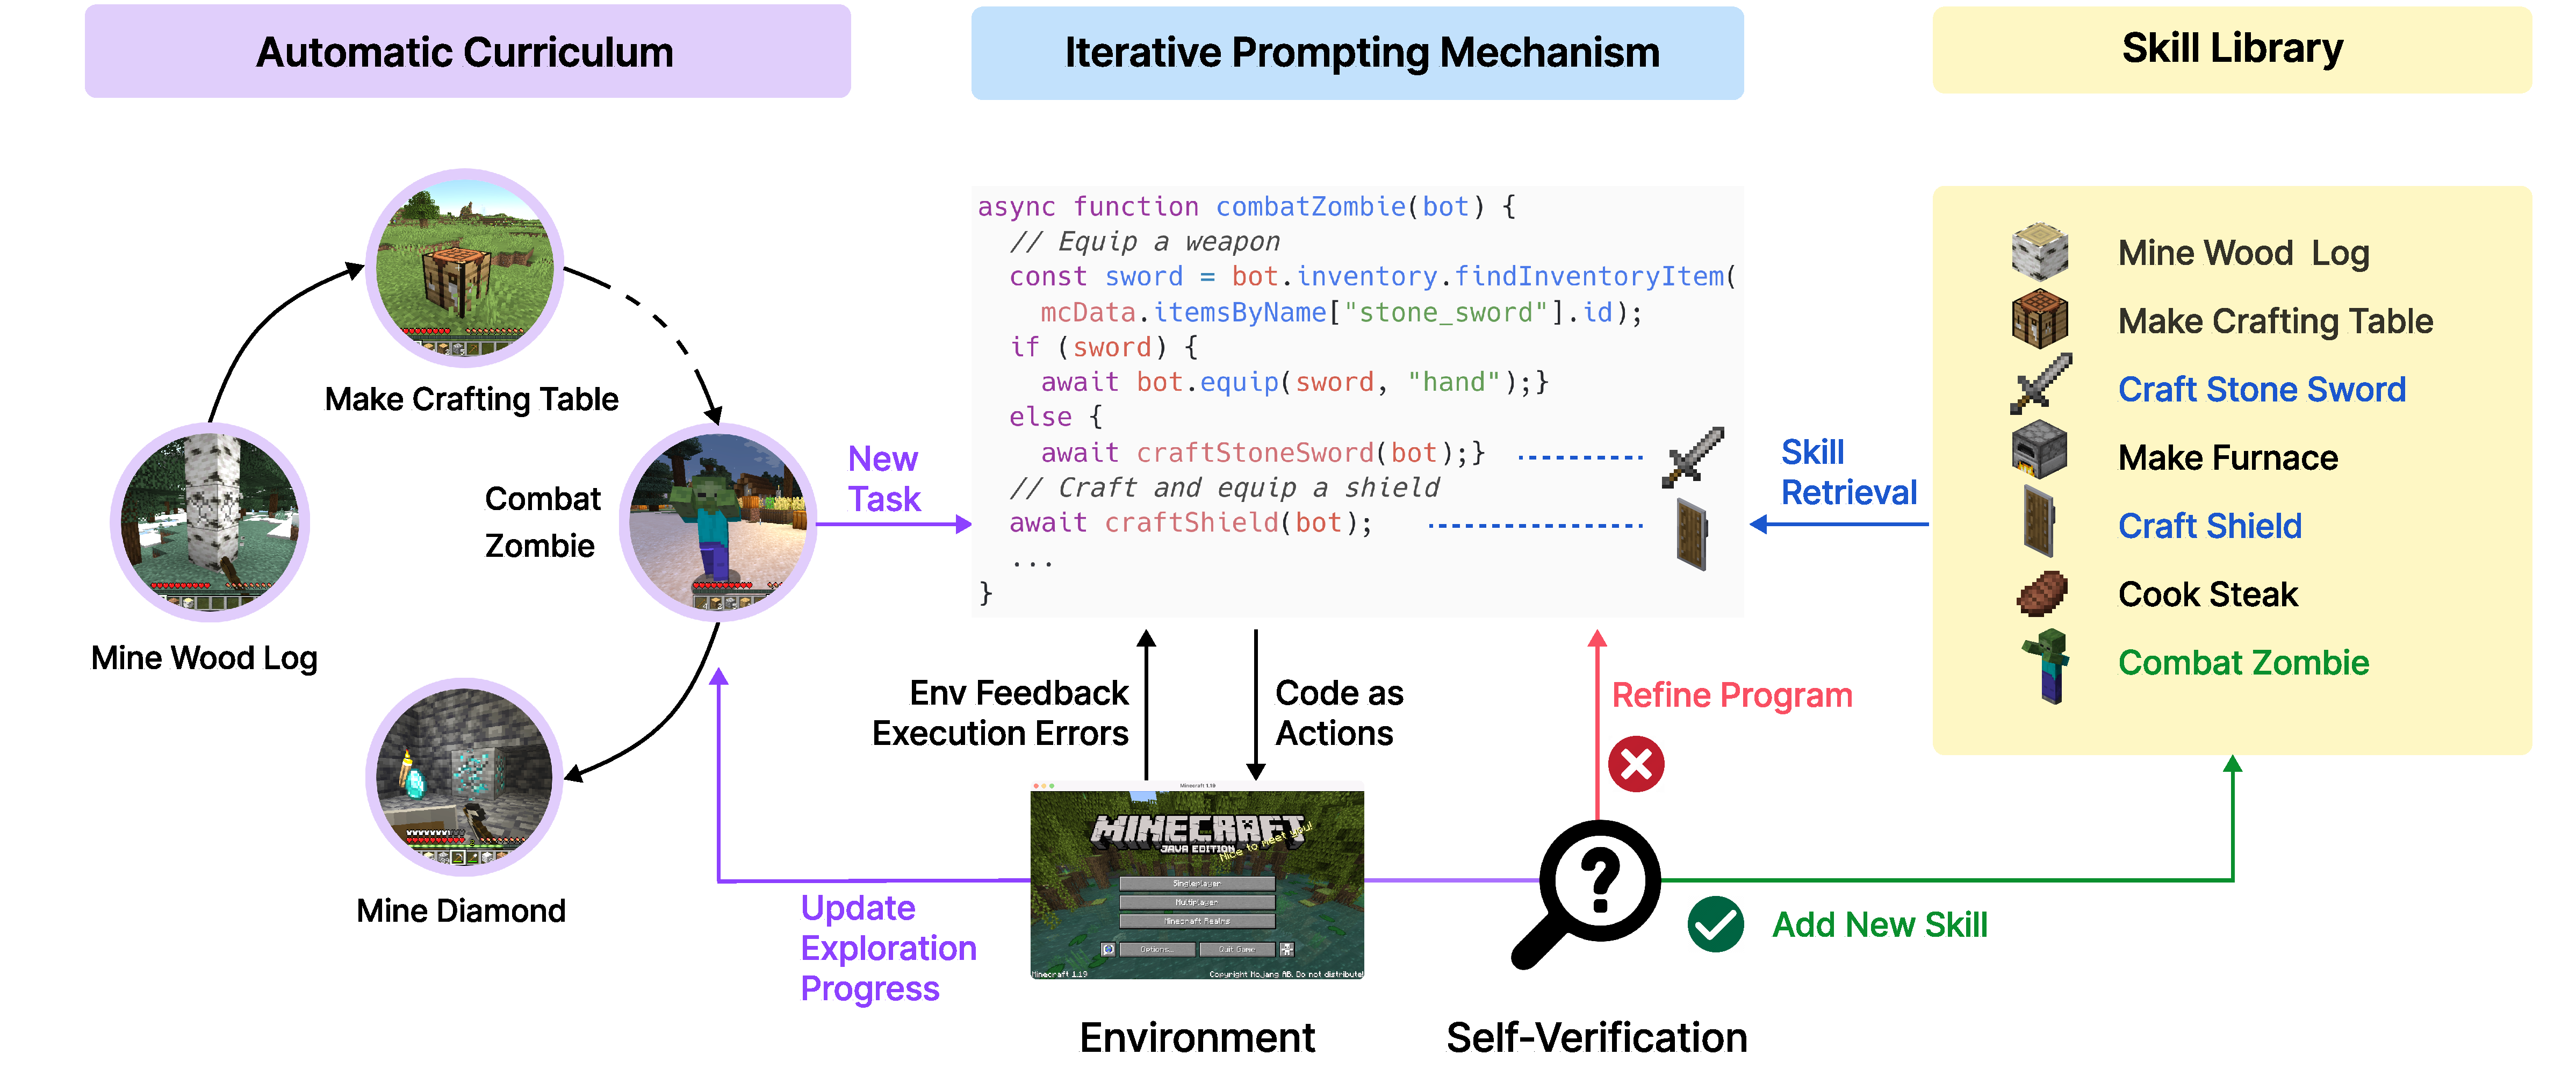
\includegraphics[width=\textwidth]{figures/pull_fig_fig.pdf}
    % \vspace{0.1em}
    \caption{\voyager consists of three key components: an automatic curriculum for open-ended exploration, a skill library for increasingly complex behaviors, and an iterative prompting mechanism that uses code as action space.}
    % \vspace{-1em}
    \label{fig:diagram}
\end{figure}


Towards these goals, we introduce \voyager, the first \textit{LLM-powered embodied lifelong learning agent} to drive exploration, master a wide range of skills, and make new discoveries continually without human intervention in Minecraft. 
\voyager is made possible through three key modules (Fig.~\ref{fig:diagram}): 1) an \textbf{automatic curriculum} that maximizes exploration; 2) a \textbf{skill library} for storing and retrieving complex behaviors; and 3) a new \textbf{iterative prompting mechanism} that generates executable code for embodied control.
We opt to use code as the action space instead of low-level motor commands because programs can naturally represent temporally extended and compositional actions~\cite{liang2022code,singh2022progprompt}, which are essential for many long-horizon tasks in Minecraft. 
\voyager interacts with a blackbox LLM (GPT-4~\cite{openai2023gpt4}) through prompting and in-context learning~\cite{wei2022emergent,brown2020gpt3,raffel2020t5}. Our approach bypasses the need for model parameter access and explicit gradient-based training or finetuning.

More specifically, \voyager attempts to solve progressively harder tasks proposed by the \textbf{automatic curriculum}, which takes into account the exploration progress and the agent's state. The curriculum is generated by GPT-4 based on the overarching goal of ``discovering as many diverse things as possible''. This approach can be perceived as an in-context form of \textit{novelty search}~\cite{eysenbach2018diversity,conti2018novelty}.
\voyager incrementally builds a \textbf{skill library} by storing the action programs that help solve a task successfully. Each program is indexed by the embedding of its description, which can be retrieved in similar situations in the future. Complex skills can be synthesized by \textit{composing} simpler programs, which compounds \voyager's capabilities rapidly over time and alleviates catastrophic forgetting in other continual learning methods~\cite{parisi2023continual,wang2023comprehensive}. 

However, LLMs struggle to produce the correct action code consistently in one shot~\cite{openai2021codex}. To address this challenge, we propose an \textbf{iterative prompting mechanism} that: (1) executes the generated program to obtain observations from the Minecraft simulation (such as inventory listing and nearby creatures) and error trace from the code interpreter (if any); (2) incorporates the feedback into GPT-4's prompt for another round of code refinement; and (3) repeats the process until a self-verification module confirms the task completion, at which point we commit the program to the skill library (e.g., \texttt{craftStoneShovel()} and \texttt{combatZombieWithSword()}) and query the automatic curriculum for the next milestone (Fig.~\ref{fig:diagram}).

Empirically, \voyager demonstrates strong \textbf{in-context lifelong learning} capabilities. It can construct an ever-growing skill library of action programs that are reusable, interpretable, and generalizable to novel tasks.
We evaluate \voyager systematically against other LLM-based agent techniques (e.g., ReAct~\cite{yao2022react}, Reflexion~\cite{shinn2023reflexion}, AutoGPT~\cite{autogpt}) in MineDojo~\cite{fan2022minedojo}, an open-source Minecraft AI framework. 
\voyager outperforms prior SOTA by obtaining $3.3 \times$ more unique items, unlocking key tech tree milestones up to $15.3 \times$ faster, and traversing $2.3 \times$ longer distances. We further demonstrate that \voyager is able to utilize the learned skill library in a new Minecraft world to solve novel tasks from scratch, while other methods struggle to generalize.
